\subsection{Host CPU}

Abbildung \ref{fig:arch_02} zeigt die Komponenten, welche für Echtzeit-Audio auf der CPU benötigt werden. Audio-Hardware muss den Digital-Analog-Wandlern einen kontinuierlichen genau-getakteten Datenstrom zuführen. Dies geschieht durch periodisches Abfragen des Betriebssystems über die Hardware-Interrupts. Die erforderliche  Puffergröße kann wenige Abtastwerte beinhalten und die Abfrageintervalle weniger als 1 ms. Dies ist abhängig von Hardware und Audio-Treibern, die verwendet wurden.

Das Betriebssystem bietet eine Abstraktionsebene in Form einer API für die Anwendungssoftware. Dies gibt der Anwendungs-Software eine einheitliche Schnittstelle, unabhängig von der Marke der Audio-Hardware und -Treiber.

Die VST-API ist eine weitere Abstraktionsebene, die wiederum eine einheitliche Schnittstelle für Plug-in-Anbieter bietet, unabhängig von der OS. Aber VST ist nicht die einzige Plug-in-API. Die JUCE-Bibliothek bietet eine eigene Plug-in-API, die einfacher ist und die Unterschiede zwischen verschiedenen Plug-in-APIs vereinheitlicht.

Die durch Interrupts der Audio-Hardware ausgelöste Datenabfrage wird durch das Betriebssystem an die DAW-Anwendung durch Rückruffunktionen weitergeleitet. Der DAW hat zuvor beim Starten die entsprechenden Rückruffunktionen an das Betriebssystem registriert. Die DAW-Anwendung ihrerseits leitet die Datenabfrage, ebenfalls durch die vom VST spezifizierten Rückruffunktionen, an alle aktiven Plug-ins weiter.

\begin{figure}[H]
    \centering
    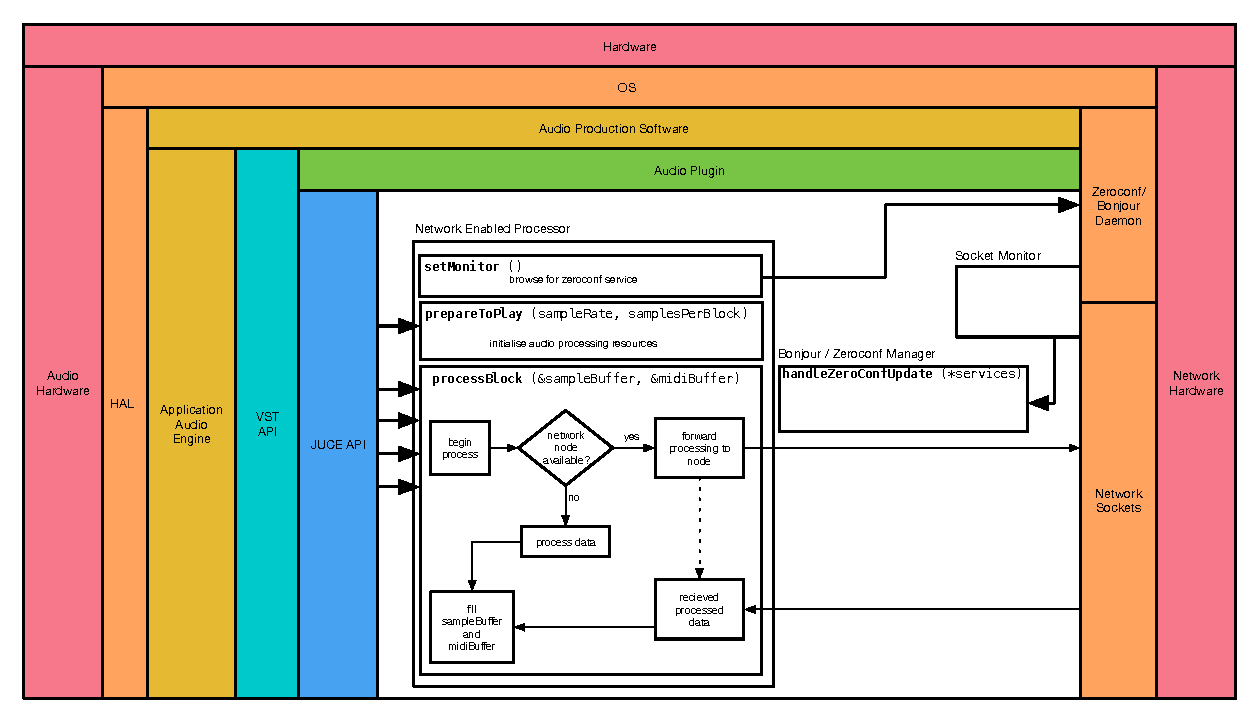
\includegraphics[width=\textwidth]{assets/architecture_02.pdf}
    \caption{Host-CPU-Überblick}
    \label{fig:arch_02}
\end{figure}

Das für dieses Projekt implementierte  Audio-Plug-in hat mehrere Netzwerkprozessoren aktiviert; in Abbildung \ref{fig:arch_02} wird nur einer als Beispiel dargestellt. Wenn das Plug-in von der Host-Software instanziiert wird, instanziiert es seinerseits jeden seiner internen Prozessoren. Die Prozessoren wiederum rufen den Bonjour / ZeroConf-Daemon des Betriebssystems auf, das Netzwerk auf einen passenden, registrierten Rechenknoten zu durchforsten. Der Aufruf geht gleichfalls an ein Socket, über welches der Daemon den Prozessor über das Auffinden eines passenden Services im Netzwerk benachrichtigen kann.

Der Bonjour / ZeroConf-Daemon zeigt dem Audio-Plug-in mittels des  Sockets eine Liste der gefundenen Services an. Das Audio-Plug-in durchsucht die Liste nach einem freien Rechenknoten. Der ausgewählte Rechenknoten wird in die ”activeNode”-Variable gespeichert.

Wenn eine Anfrage für Audio-Daten von der DAW-Anwendung an das Plug-in übergeben wird, dann wird die „processBlock”-Funktion des Plug-ins aufgerufen. Das Plug-in seinerseits ruft die „processBlock”-Funktionen jeden seiner internen Audio-Prozessoren nacheinander auf. In Abbildung \ref{fig:arch_02} wird dies vereinfacht dargestellt mit der „processBlock”-Funktion eines einzigen Audio-Prozessors. Der „processBlock”-Funktion wird eine Referenz zugeteilt bezüglich der aktuellen, zu verarbeitenden Audiopuffer und MIDI-Puffer. Der Audiopuffer enthält die einzelnen Audioabtastungen für jeden Kanal als Float-Werte. Der MIDI-Puffer enthält Performance-Daten wie die Eintrittszeit und Tonhöhe der gespielten Noten.

Innerhalb der „processBlock”-Funktion prüft der Prozessor, ob ein Rechenknoten im ”activeNode” gespeichert ist. Wenn ja, dann leitet er sofort die MIDI- und Audiodaten sowie die eigenen Zustandsdaten an den Rechenknoten und wartet auf die Antwort. Wenn die Antwort eintrifft, werden die Daten zurück in die entsprechenden Puffer kopiert. Die DAW-Anwendung fragt die nächsten Plug-ins dann weiter ab, bis die gesamte Verarbeitungskette abgeschlossen ist. Die resultierenden Puffer werden an die Audiohardware über die HAL API geschickt.